\subsection{Glyph: \glyph{Unspecified entity}}
\label{sec:unspecifiedEntity}

The simplest type of EPN is the \glyph{unspecified entity}: one which type is unknown or simply not relevant to the purposes of the map. This arises, for example, when the existence of the entity has been inferred indirectly, or when the entity is merely a construct introduced for the needs of a map, without direct biological equivalent.  For cases where the identity of the entities composing the pool \emph{is} known, there exist other, more specific glyphs described below in the manual.

An \glyph{unspecified entity} is represented by an elliptic container, as shown in \fig{unspecified}.  Note that this
must remain an ellipse to avoid confusion with the Simple Chemical glyph, which is a circle (c.f.\, \ref{sec:simpleChemical}).

\begin{figure}[H]
  \centering
  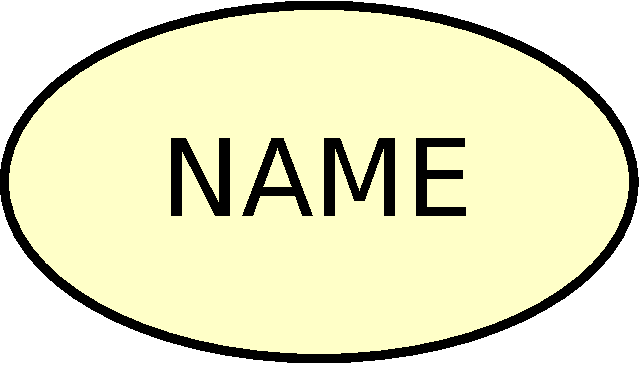
\includegraphics[scale = 0.3]{images/unspecified}
  \caption{The \PD glyph for \glyph{unspecified entity}.}
  \label{fig:unspecified}
\end{figure}

